\NeedsTeXFormat{LaTeX2e}
%\PassOptionsToClass{handout}{beamer}
\documentclass{beamer}
\usepackage{beamerPack}
\usepackage[boxed,ruled,vlined]{algorithm2e}
\usetikzlibrary{shapes.geometric,arrows,fit,matrix,positioning}
\tikzset{
  treenode/.style = {circle, draw=black, align=center, minimum size=1cm, anchor=center},
  subtree/.style = {regular polygon, regular polygon sides=3, draw=black, align=center, minimum height=0.8cm, minimum width=0.6cm, anchor=north}
}
\usepackage[03]{../lecture}
\subtitle{整列}
\begin{document}

\begin{frame}[fragile]{}
\titlepage
\end{frame}

\section{Sorting}		%%%%%%%%
\subsection{}

\begin{frame}[fragile]{整列}{}
\begin{itemize}\itemindent15mm\labelsep10mm
\item[初期状態]入力: 配列\texttt{VecT}

\medskip
\scalebox{0.6}{
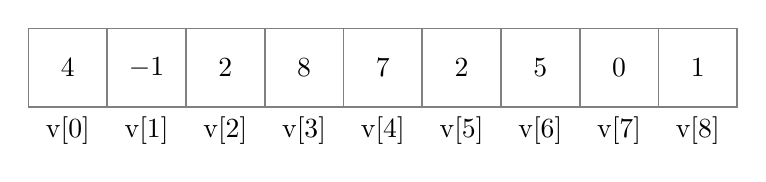
\begin{tikzpicture}[
    , cell/.style = {rectangle,draw=gray,semithick,minimum size=1cm,outer sep = 0mm,label=below:v{[\j]}}
]
\foreach \i [count=\j from 0] in {4, -1, 2, 8, 7, 2, 5, 0, 1}
    \node[cell] at (\j, 0) {$\i$};
\end{tikzpicture}
}
\item[最終状態]出力: 整列ずみの配列\texttt{VecT}

\medskip
\scalebox{0.6}{
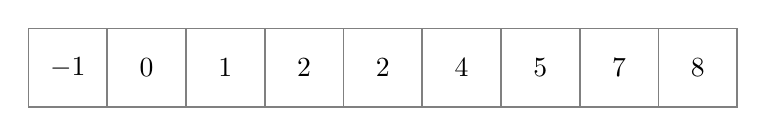
\begin{tikzpicture}[
    , cell/.style = {rectangle,draw=gray,semithick,minimum size=1cm,outer sep = 0mm}
]
\foreach \i [count=\j from 0] in {-1, 0, 1, 2, 2, 4, 5, 7, 8}
    \node[cell] at (\j, 0) {$\i$};
\end{tikzpicture}
}
\end{itemize}
全ての要素に順序がつけられること:全順序性が必要。
\end{frame}

\section{Bubble sort}		%%%%%%%%
\subsection{}

\begin{frame}[fragile]{バブルソート}{}
\scalebox{0.5}{
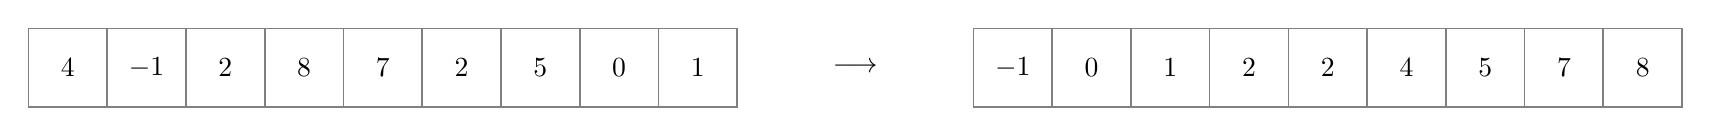
\begin{tikzpicture}[xshift=0.15\textwidth
    , cell/.style = {rectangle,draw=gray,semithick,minimum size=1cm,outer sep = 0mm}
]
\foreach \i [count=\j from 0] in {4, -1, 2, 8, 7, 2, 5, 0, 1}
    \node[cell] at (\j, 0) {$\i$};
\node at (10, 0) {$\longrightarrow$};
\foreach \i [count=\j from 0] in {-1, 0, 1, 2, 2, 4, 5, 7, 8}
    \node[cell] at (\j + 12, 0) {$\i$};
\end{tikzpicture}
}

\vfill
適切な中間目標を設定せよ

\vfill
先頭の1個が要件を満たしている

\vfill
\scalebox{0.6}{
\begin{tikzpicture}[cell/.style = {rectangle,draw=gray,semithick,minimum size=1cm,outer sep = 0mm}]
\foreach \i [count=\j from 0] in {-1, 0, 1, 2, 2, 4, 5, 7, 8}
    \node[cell] at (\j, 0) {$\i$};
\node[anchor=west] at (9,0) {中間目標になってない};
\end{tikzpicture}
}

\medskip
\scalebox{0.6}{
\begin{tikzpicture}[cell/.style = {rectangle,draw=gray,semithick,minimum size=1cm,outer sep = 0mm}]
\foreach \i [count=\j from 0] in {-1, 0, 0, 0, 0, 0, 0, 0, 0}
    \node[cell] at (\j, 0) {$\i$};
\node[anchor=west] at (9,0) {次のステップにいけない};
\end{tikzpicture}
}

\medskip
\scalebox{0.6}{
\begin{tikzpicture}[cell/.style = {rectangle,draw=gray,semithick,minimum size=1cm,outer sep = 0mm}]
\foreach \i [count=\j from 0] in {-1, 5, 2, 2, 8, 4, 0, 7, 1}
    \node[cell] at (\j, 0) {$\i$};
\node[anchor=west] at (9,0) {順番が変わってしまった。問題か?};
\end{tikzpicture}
}

\medskip
\scalebox{0.6}{
\begin{tikzpicture}[cell/.style = {rectangle,draw=gray,semithick,minimum size=1cm,outer sep = 0mm}]
\foreach \i [count=\j from 0] in {-1, X, X, X, X, X, X, X, X}
    \node[cell] at (\j, 0) {$\i$};
\node[anchor=west] at (9,0) {$X$は-1以外のもとからあった要素};
\end{tikzpicture}
}
\end{frame}

\begin{frame}[fragile]{バブルソートの構造}{}
並びの順に、
\begin{itemize}%\itemsep8pt
\item 中間目標を解いて要件を満たす範囲(区間)を拡大
\item 対象範囲を縮小(相似問題に帰着)
\end{itemize}

\vfill
\begin{itemize}%\itemsep8pt
\item 中間目標=先頭要素は範囲内の最小値であること(探索という既知のアルゴリズムの応用)
\item 停止性:対象範囲は単調減少なので必ず終了
\end{itemize}
\end{frame}

\begin{frame}[fragile]{バブルソート}{}
\begin{tikzpicture}[
    overlay
    , xshift=0.5\textwidth
]
\node[] at (8,-3) {\pgfimage[height=0.9\pagewidth]{alberto-bianchini-krPdyjs1iTM-unsplash.jpg}};
\node[color=gray,rotate=90] at (6.2,-4) {\fontsize{4}{4}\selectfont Photo by Alberto Bianchini on Unsplash};
\draw[draw=blue!4,fill=blue!4,rounded corners=3,anchor=west] (-5.2,-4.8) rectangle ++(+7, +1.8) {};
\end{tikzpicture}

\begin{algorithm}[H]
\KwIn{v: \texttt{Vec<T>}--対象配列}
\KwIn{start: Int -- 対象範囲の下限}
\KwIn{end: Int -- 対象範囲の上界(上限+1)}
\SetKwComment{Comment}{}{}
\BlankLine
\If{startがendと等しい}{
  \Return{}
}
\For{iをend の直前からstartの直前まで}{
    \If{v[i-1] > v[j]}{
      v[i-1] と v[i] とを入れ替える\;
    }
}
\Return{startを1増やして再帰呼び出し}
\caption[page]{再帰版バブルソート}
\end{algorithm}
\vfill
if文, for文、入れ替え、再帰呼び出し。探索と同じくif文の実行回数で評価。
\end{frame}

\begin{frame}[fragile]{バブルソートRust版}{}
\begin{codeof}{language=Rust}{bsort.rs}
pub fn bsort<T: Ord>(v: &mut [T]) {
    if v.len() == 0 { return; }
    for i in (1..v.len()).rev() {
        if v[i - 1] > v[i] {
            v.swap(i - 1, i);
        }
    }
    bsort(&mut v[1..])
}
\end{codeof}

引数が多くなると行が長くなって見苦しいのでスライスを使用した。

\end{frame}

\begin{frame}[fragile]{再帰関数の計算量評価}{}

\begin{columns}[T]
\begin{column}{0.5\textwidth}
\begin{codeof}{language=Rust}{bsort}
fn bsort(長さ\@N@) {
  長さ\@N@の最小値探索;
  bsort(長さ\@N-1@);
\end{codeof}
\end{column}
\begin{column}{0.5\textwidth}
\begin{align*}
T(n) = & n + T(n-1)\\
= & n + (n - 1) + \cdots + 1 \\
T(N) = & O(N^2)
\end{align*}
\end{column}
\end{columns}

\begin{columns}[T]
\begin{column}{0.5\textwidth}
\begin{codeof}{language=Rust}{再帰版lsearch}
fn lsearch(長さ\@N@,c) {
  c();
  lsearch(長さ\@N-1@, c);
\end{codeof}
\end{column}
\begin{column}{0.5\textwidth}
\begin{align*}
T(n) = & 1 + T(n-1)\\
= & n \times O(1) \\
T(N) = & O(N)
\end{align*}
\end{column}
\end{columns}

\begin{columns}[T]
\begin{column}{0.5\textwidth}
\begin{codeof}{language=Rust}{再帰版bsearch}
fn bsearch(長さ\@$N$@, c) {
  c();
  bsearch(長さ\@$N/2$@, c);
\end{codeof}
\end{column}
\begin{column}{0.5\textwidth}
\begin{align*}
T(n) = & 1 + T(n/2)\\
= & 1 \times O(\log(n)) \\
T(N) = & O(\log(N))
\end{align*}
\end{column}
\end{columns}
\end{frame}

\section{Quick sort}		%%%%%%%%
\subsection{}

\begin{frame}[fragile]{第2のアイデア}{}
\begin{tikzpicture}[overlay, xshift=0.5\textwidth]
\node[] at (-3.5,-6) {\pgfimage[width=0.5\pagewidth]{jigzaw-1.jpg}};
\node[] at ( 3.5,-6) {\pgfimage[width=0.5\pagewidth]{jigzaw-2.jpg}};
\end{tikzpicture}
\scalebox{0.5}{
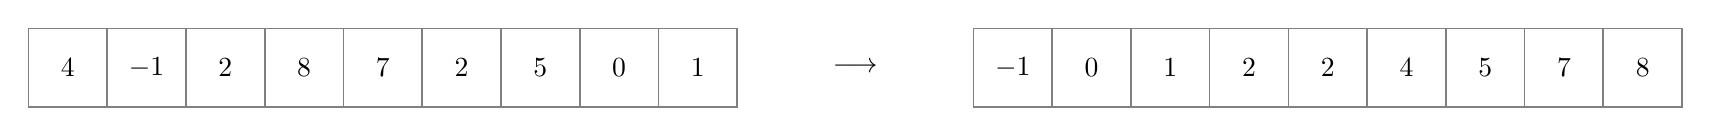
\begin{tikzpicture}[xshift=0.15\textwidth
    , cell/.style = {rectangle,draw=gray,semithick,minimum size=1cm,outer sep = 0mm}
]
\foreach \i [count=\j from 0] in {4, -1, 2, 8, 7, 2, 5, 0, 1}
    \node[cell] at (\j, 0) {$\i$};
\node at (10, 0) {$\longrightarrow$};
\foreach \i [count=\j from 0] in {-1, 0, 1, 2, 2, 4, 5, 7, 8}
    \node[cell] at (\j + 12, 0) {$\i$};
\end{tikzpicture}
}

\vfill
適切な中間目標:N/2個のソート問題ふたつに帰着
\begin{itemize}%\itemsep8pt
\item 他方のどの要素よりも小さい要素だけからなる配列
\item 他方のどの要素よりも大きい要素だけからなる配列
\end{itemize}
それぞれを整列、順につなげば全体が整列
\vfill
\end{frame}

\begin{frame}[fragile]{クイックソートアルゴリズム}{}
\begin{algorithm}[H]
\KwIn{v: \texttt{Vec<T>}--対象配列}
\KwIn{start, end -- 対象範囲}
\SetKwComment{Comment}{}{}
\BlankLine
\If{startがendと等しい}{
  \Return{}
}
m = 適当な値\;
vの要素でm以下のものを左に、大きいものを右にまとめる\;
p = 境目の添字\;
v, start, pを引数に再帰呼び出し\;
v, p, endを引数に再帰呼び出し\;
\Return{}
\caption[page]{クイックソート}
\end{algorithm}

\vfill
{\fontsize{9}{9}\selectfont
コピーを作らずその場で並べ替えているので、できたものを「つなぐ」必要がない(in-place search)。
}
\end{frame}

\begin{frame}[fragile]{クイックソートRust版下請け関数}{}
\begin{codeof}{language=Rust}{配列を二つに分割(または長さ$N$の配列の並べ替え)}
fn partition<T: Ord>(v: &mut [T]) -> usize {
    let mut i = 0;      // 小さなものを移動させた総数
    for j in (0..v.len()).rev() {
        if v[j] <= v[v.len() - 1] {
            v.swap(i, j);
            i += 1;  // +1したので次に小さなものを入れるべき添字
        }
    }
    i   // 小さいものの総数(あるいは最後の小さいものの添字+1)
}
\end{codeof}
\vfill
適当な値$m$として配列の最後の要素v[v.len()-1]を採用した。
\end{frame}

\begin{frame}[fragile]{qsort (qsort.rs)}{}
\begin{codeof}{language=Rust}{quick sort}
pub fn qsort<T: Ord>(v: &mut [T]) {
    if v.len() <= 1 { return; }
    let p = partition(v);
    qsort(v[0..p]);     // vの前半分
    qsort(v[p..]);      // vの後半分
}
\end{codeof}
\end{frame}

\begin{frame}[fragile]{クイックソートの計算量評価}{最悪計算量、最良計算量、平均計算量}
\begin{columns}[T]
\begin{column}{0.5\textwidth}
\begin{codeof}{language=Rust}{qsort}
fn qsort(長さ\@N@) {
  長さ\@N@の並べ替え;
  qsort(長さ\@N/2@);
  qsort(長さ\@N/2@);
\end{codeof}
\end{column}
\begin{column}{0.5\textwidth}
\begin{align*}
T(n) = & ? + T(n/2) + T(n/2) \\
     = & n + 2T(n/2) \\
     = & n \times \log(n) \\
T(N) = & O(N\log(N))
\end{align*}
\end{column}
\end{columns}

\vfill

\begin{columns}[T]
\begin{column}{0.5\textwidth}
木の深さごとに計算量を小計
{
\fontsize{9}{10}\selectfont
\begin{tabular}[h]{| r | r | r |}
\CH 深さ & 作業内容 & 個数 \\
\CL $1$ & N個の並べ替え & $1$ \\
\CL $2$ & $N/2$個の並べ替え & $2$ \\
\CL $3$ & $N/4$個の並べ替え & $4$ \\
\CL $\log_2(N)$ & $1$個の並べ替え & $N$ \\
\end{tabular}
}
\end{column}

\begin{column}{0.5\textwidth}
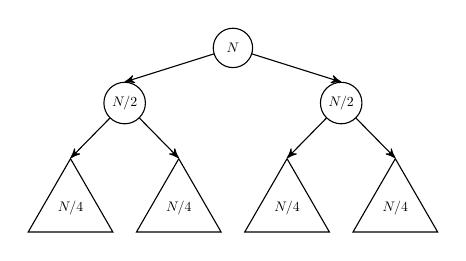
\begin{tikzpicture}[->,>=stealth',level/.style={sibling distance = 5.5cm/#1, level distance = 1.4cm},scale=0.5, transform shape]
\node [treenode] {$N$}
    child[child anchor=north] { node[treenode] {$N/2$}
        child[child anchor=north] { node [subtree] {$N/4$} }
        child[child anchor=north] { node [subtree] {$N/4$} }
    }
    child[child anchor=north] { node[treenode] {$N/2$}
        child[child anchor=north] { node [subtree] {$N/4$} }
        child[child anchor=north] { node [subtree] {$N/4$} }
    }
    ;
\end{tikzpicture}
\end{column}
\end{columns}

\end{frame}

\section{Summary}		%%%%%%%%
\subsection{}

\begin{frame}[fragile]{ソートアルゴリズムの比較}{\href{https://www.geogebra.org/graphing}{\beamergotobutton{geogebra}}}

{%\fontsize{9}{10}\selectfont
\begin{tabular}[h]{|l|r|r|r|}
\CH アルゴリズム & 時間計算量 & 空間-- & 安定 \\
\CL バブルソート & $O(N^2)$ & $O(1)$ & \checkmark\\
\CL クイックソート & $O(N\log(N))$ & $O(\log(N))$ & \\
\CL ヒープソート & $O(N\log(N))$ & $O(\log(N))$ & \checkmark \\
\CL マージソート & $O(N\log(N))$ & $O(\log(N))$ & \checkmark \\
\end{tabular}
}

\vfill
今回話さなかったこと:{\bf 2分割できるとは限らない}
\begin{itemize}%\itemsep8pt
\item 要素数が極めて少ない時はバブルソートを使う
\item スタックの消費を嫌って途中からヒープソート
\end{itemize}

\vfill
ヒープソート:データ構造ヒープにデータを登録($O(\log(N))$)、ヒープから取り出し($O(\log(N))$)
\end{frame}

\begin{frame}[fragile]{マージソート}{}
データを二分。再帰的に処理して整列する、それぞれストリームとみなして一つに合成、マージ、整流、zip。

\begin{codeof}{language=Rust}{二つのストリームを第3のストリームにマージする}
fn merge(a: mut stream, b: mut stream, c: stearm) {
    while a.is_empty() && b.is_empty() {
        if aの先頭 < bの先頭 {
          c.push(a.pop());
          if aが空になった { c.append(b); return; }
        } else {
          c.push(b.pop());
          if bが空になった { c.append(a); return; }
        }
    }
}
\end{codeof}
この処理は$O(N)$。全体として$T(n)= T(n/2) + T(n/2) + n$
\end{frame}

\begin{frame}[fragile]{ここまでの振り返り}{アルゴリズム=自明または「前処理$\to$相似問題$\to$後処理」}

{
%\fontsize{9}{10}\selectfont
\begin{tabular}[h]{r l}
\CL 1つを処理、残りを再帰  & $T(n) = 1 + T(n-1) + 0$ \\
\CL 1つを処理、残りを再帰  & $T(n) = 1 + T(n/2) + 0$ \\
\CL 1つを処理、残りを再帰  & $T(n) = n + T(n-1) + 0$ \\
\CL 再帰の準備、再帰、再帰 & $T(n) = n + T(n/2) + T(n/2) + 0$ \\
\CL 再帰、再帰、結果の合成 & $T(n) = 0 + T(n/2) + T(n/2) + n$ \\
\end{tabular}
}

\vfill
これまでの全ての問題において、
\begin{itemize}%\itemsep8pt
\item 中間目標の設定・帰納的構造の発見が、問題を解けることに
\item 再帰関数を定義できることが、プログラムを作れることに
\end{itemize}

対応する。
\end{frame}

\begin{frame}[fragile]{}{}
{
\fontsize{11}{11}\selectfont
中学数学の「式を立てる」と同様の「アルゴリズムを立てる」スキルが必要。
}

\begin{tcolorbox}[colframe=white,colback=black!2!white]
\fontsize{8}{10}\selectfont
\begin{quotation}
「プログラミング的思考」は、文部科学省によると「自分が意図する一連の活動を実現するために、どのような動きの組合せが必要であり、一つ一つの動きに対応した記号を、どのように組み合わせたらいいのか、記号の組合せをどのように改善していけば、 より意図した活動に近づくのか、といったことを論理的に考えていく力」と定義されています。
\end{quotation}
\end{tcolorbox}

{
\fontsize{11}{11}\selectfont
その上で立てたものを解くスキルが必要。
}

\end{frame}

\begin{frame}[fragile]{}{}
\begin{center}
\pgfimage[width=0.85\pagewidth]{tekishikou.png}
\end{center}

\begin{tcolorbox}[colframe=white,colback=black!2!white]
\fontsize{6}{8}\selectfont
\begin{quotation}
そして、「すでにコンピューターを使ったプログラミングをやっているよ」という方もぜひ、この番組をご覧ください。プログラミング的思考を育むことで、プログラミングがより上手になるのはもちろん、プログラミング以外の普遍的なシーンでも、その考え方を役立てることができます。
\end{quotation}
\end{tcolorbox}
\end{frame}
\end{document}
